\documentclass[aps,pre,reprint,superscriptaddress,amsmath,amssymb,nofootinbib]{revtex4-1}
\usepackage{graphicx}
\usepackage{dcolumn}
\usepackage{bm}
\usepackage{hyperref}
\usepackage{natbib}
\renewcommand{\thefootnote}{\fnsymbol{footnote}}
\DeclareGraphicsExtensions{.pdf}
\renewcommand\thesection{\arabic{section}}
\renewcommand\thesubsection{\arabic{section}.\arabic{subsection}}

\makeatletter
\def\p@subsection{}
\makeatother

\begin{document}


\title{Spatially embedded growing small-world networks}
\author{Ari Zitin}
\affiliation{Institute for Research in Electronics and Applied Physics, University of Maryland, College Park, Maryland 20742, USA}
\author{Alex Gorowara}
\affiliation{Institute for Research in Electronics and Applied Physics, University of Maryland, College Park, Maryland 20742, USA}
\author{Shane Squires}
\affiliation{Institute for Research in Electronics and Applied Physics, University of Maryland, College Park, Maryland 20742, USA}
\affiliation{Department of Physics, University of Maryland, College Park, Maryland 20742, USA}
\author{Mark Herrera}
\affiliation{Institute for Research in Electronics and Applied Physics, University of Maryland, College Park, Maryland 20742, USA}
\affiliation{Department of Physics, University of Maryland, College Park, Maryland 20742, USA}
\author{Tom Antonsen}
\affiliation{Institute for Research in Electronics and Applied Physics, University of Maryland, College Park, Maryland 20742, USA}
\affiliation{Department of Electrical and Computer Engineering, University of Maryland, College Park, Maryland 20742, USA}
\affiliation{Department of Physics, University of Maryland, College Park, Maryland 20742, USA}
\author{Michelle Girvan}
\affiliation{Institute for Research in Electronics and Applied Physics, University of Maryland, College Park, Maryland 20742, USA}
\affiliation{Institute for Physical Science and Technology, University of Maryland, College Park, Maryland 20742, USA}
\affiliation{Department of Physics, University of Maryland, College Park, Maryland 20742, USA}
\author{Edward Ott}
\affiliation{Institute for Research in Electronics and Applied Physics, University of Maryland, College Park, Maryland 20742, USA}
\affiliation{Department of Electrical and Computer Engineering, University of Maryland, College Park, Maryland 20742, USA}
\affiliation{Department of Physics, University of Maryland, College Park, Maryland 20742, USA}

\date{\today}

\begin{abstract}
Networks in nature are often formed within a spatial substrate in a dynamical manner, gaining links and nodes as they develop over time. 
Motivated by biological considerations, we propose a class of spatially-based growing network models and investigate the relationship between the resulting statistical network properties and the space in which the networks are embedded. 
In particular, we consider models in which nodes are placed one by one in random locations in space, with each such placement followed by configuration relaxation toward uniform node density, and connection of the new node with spatially nearby nodes. 
We characterize the spatial and topological properties of these networks and show how spatial embedding supports the emergence of small-world networks.
\end{abstract}

\pacs{05.45.-a, 05.65.+b, 89.75.-k, 89.75.Fb ,89.75.Hc} %Nonlinear dynamics and chaos, Self-organized systems, Complex Systems, Structures and organization in complex systems, Networks and genealogical trees

\maketitle

\section{INTRODUCTION}
%in the introduction don't forget to present definitions we use, in particular be clear what we mean by small world property
%mention how our generalizations were chosen for their physical significance rather than the ease with which we can perform comupational and analytic calculations of their properties. 
The burgeoning field of network science has made significant headway in the past 15 years exploring the statistical properties and growth processes of real world complex networks.
The identification of the small-world property by Watts and Strogatz in \cite{wsnat} represented a significant step towards understanding the underlying structure of many existing networks.
Small-world networks exhibit two key properties, the first being a short characteristic path length similar to an Erd\H{o}s-R\'{e}nyi random network, and the second being a high clustering coefficient.
More specifically, the characteristic path length ($\ell$), which is the average over all nodes of the smallest number of links connecting a pair of nodes, must grow no faster than $\log N$ where $N$ is the size of the network (i.e. $\ell \sim \log N$).
In this paper we define the clustering coefficient to be the number of closed triplet divided by the number of connected triples of vertices, i.e. the fraction of triples that form complete triangles \cite{newmanrandom}.
In order for a network to have the small-world property we require that this clustering coefficient approach some non-zero value for large $N$.
Real world networks from the social networks to networks of neurons exhibit the small-world property, revealing it as something fundamental about the structure of many networks.

Another key feature of real world networks is that they often live in some physical space with imposed spatial contraints. 
E.g., the Internet, a network of routers connected via cables, is embedded on the $2$-dimensional surface of the Earth and can only have links of a certain physical distance due to the cost of wiring.
This has led many researchers to consider network models with spatial embedding \cite{ozik2004,przuljgeo,hermannspace,bullockspatial,guan1D,zhang2006,zhang2007}.
Work on this topic has revealed that spatially constrained networks can lead to small-world networks, even when links are only formed locally.
Many of these models (e.g. \cite{bullockspatial,guan1D,przuljgeo}) introduce growing network models, but force the nodes to remain fixed in their initial spatial location.
Of the literature on the subject, only \cite{ozik2004} introduces a growing network model in which nodes can move once placed in a spatial substrate.
The importance of dynamics in the growth of the network cannot be understated, real world networks are often dynamic in both time and space, with new nodes being added while existing nodes are free to move about.
For example social networks generally require spatial proximity to form (people tend to make friends with those near them), but people don't stay still, in fact many of the critical features of social networks arise from the fact that people in the modern era are able to travel across the globe with ease. 
As such, we seek to further the work performed in \cite{ozik2004} by introducing a class of growing network models that have spatially contrained nodes free to move about in the embedding surface. 

Models of spatially embedded networks have been used previously to attempt to describe real world networks, from the neuronal networks of the \textit{C. Elegans} worm \cite{plenzcascade} to the protein interaction network of the common fruit-fly \cite{fruitfly}, biological researchers have used network theory to describe physically embedded networks.
Further applications of spatial network models are presented in \cite{neuronembedding,barthelemy,vazquez2002}.
This motivates us to explore how networks depend on the space in which we embed them, and what features of this space are most important in determining network properties.

\section{THE CIRCLE MODEL}
In Ref. \cite{ozik2004} the authors presented a model, henceforth referred to as the Circle Mode, which considers a network which initially has $m+1$ uniformly separated, all-to-all connected nodes on the circumference of a circle. 
At each discrete time step the network is grown according to the following rules: 
(1) a new node is placed at a randomly selected point on the circumference of the circle;
(2) the new node is linked to its $m$ nearest neighbors;
(3) preserving node positional ordering, the nodes are repositioned to make the nearest-neighbor distance uniform;
(4) steps (1-3) are repeated until the network has $N$ nodes.
Since the network is incremented in size by one node each time step, the network size $N$ can also be used as the system time parameter.  
It has been shown \cite{ozik2004} that this growth model leads to a small-world network with an exponentially decaying degree distribution. 
The original goal of the Circle Model was to explore the effect that geographic attachment locality has on the growth of networks.
In this paper, we extend this analysis by considering networks growing by geographic attachment preference in more general spaces. 

We defined a network growth procedure to yield the small-world property if, as $N \to \infty$,
(i) the average degree $\langle k \rangle$ of a node approaches a non-zero value,
(ii) the characteristic graph path length (defined as the average value of the smallest number of links joining node pairs) does now grow with $N$ faster than $\log N$, and
(iii) the clustering coefficient (defined below) does not approach zero.
The original Circle Model exhibits these properties.
\begin{itemize}
  \item \textbf{Degree Distribution:} The degree distribution $H(k)$ is the probablility that a randomly selected node has $k$ network connections at time $N$.
For large $N$, the degree distribution of the Circle Model is given by 
\begin{equation}\label{degdist}
H(k) = \frac{1}{m+1}\left(\frac{m}{m+1}\right)^{k-m}
\end{equation},
for $k \geq m$, and $H(k) = 0$ for $k < m$ \cite{ozik2004}.
Since the number of new links added each time a new node is added is $m$, Eq. \eqref{degdist} yields the result that, the average node degree $\langle k \rangle$ is $2m$, satisfying the criterion (i) for the small-world property.
  \item \textbf{Characteristic Path Length:} In the Circle Model, simulation results show the path length scaling, $\ell \sim \log N$ [criterion ii].
This may be explained intuitively by noting that as new nodes are added they push apart the older connected nodes, lengthening the spatial distance traversed by older edges. 
These older nodes can then have geographically long links, thus dramatically decreasing the shortest graph path length between any given pair of nodes.
  \item \textbf{Clustering Coefficient:} For the Circle Model it was shown  that the clustering coefficient approaches a constant, positive, $m$-dependent value as $N \to \infty$ [criterion (iii)]. 
The clustering coefficient of a network is the fraction of connected triples which are also triangles.
This measures whether two nodes which are both connected to a third node are likely to be connected to one another. \footnote{In \cite{ozik2004} an alternate definition of clustering was used, specifically, the average of the local clustering $C_i$ of each node, $C_i = q_i/[\frac{1}{2} k_i (k_i-1)]$ where $q_i$ is the number of links between the $k_i$ neighbors of node $i$.}
\end{itemize}
The Circle Model, being fundamentally based upon the supposed one-dimensional and spatial periodicity of the underlying space (a circle), naturally raises the question of whether similar properties apply for other types of underlying spaces, e.g., spaces with higher dimensionality. 
The goal of this paper is to address this question.

\section{THE SPHERE NETWORK MODEL}
One natural generalization from embedding nodes on the one-dimensional circumference of a circle is to embed them on the two-dimensional surface of a sphere, or in general on the $d$-dimensional surface of a hypersphere ($d=1$ corresponding to the CircleModel).
On a circle it is trivial to arrange $N$ points along the circumference with uniform spacing, but the analogous procedure is less well-defined on higher dimensional surfaces.
One way to generalize the arrangement procedure is to consider nodes to be point charges and to move them to a minimum electrostatic energy equilibrium configuration. 
The problem of finding the equilibrium configuration of point charges on the surface of a sphere dates back to 1904 when J.J. Thomson introduced his model of the atom, and the problem of obtaining such an equilibrium is sometimes referred to as the `Thomson problem' \cite{thomson1904}. A related `Generalized Thomson problem' assumes that the force between `charges' is proportional to $r^{-\alpha}$ with $\alpha$ not necessarily equal to the Couloumb value, $\alpha = d$ \cite{nelson}. In general, our numerical simulations show that results for network properties are independent of $\alpha$ (Sec. \ref{sub:forcelaw}), and most of our simulations use $\alpha = d-1$.

Using the generalized Thomson problem as a guide, we develop one of our generalizations to the Circle Model, which we call the Sphere Network Model, as follows.
We model the nodes as point charges confined to the surface of a $d$-sphere of unit radius.
At each time step, we drop a new node onto the sphere at random with uniform probability density per unit area and then add links to connect it to its $m$ nearest neighbors, where distance is defined as the shortest great circle path along the surface of the sphere between two nodes.
Next we minimize the potential energy of the configuration by a steepest descent procedure, 
\begin{equation}
d\textbf{x}_i/dt = -P\{\textbf{F}_i\},\\
\textbf{F}_i = \sum_{i \neq j} \frac{(\textbf{x}_i - \textbf{x}_j)}{|\textbf{x}_i - \textbf{x}_j|^{\alpha}},
\end{equation}
where $\textbf{x}_i$ is the $(d+1)$ dimensional position vector of node $i$, $|\textbf{x}_i| \equiv 1$, and $P\{...\}$ denotes projection onto the $d$-dimensional surface of the sphere.
Note that, as new nodes are added, this procedure tends to yield a local energy minimum, as opposed to the global minimum, and we view this as being appropriate for the situations of interest to us (e.g., biological network growth processes).
For large $N$, the repulsive interaction ensures that the points are distributed approximately uniformly on the surface of the $d$-sphere.
In this way we reproduce the key features of the Circle Model in a higher dimensional space.

As a result of the Couloumb interaction, the minimum energy configuration for these points on the sphere is one where the points are distributed in an approximately uniform manner on the surface of the sphere.
In order to check if this model produces a small world network we determine the following three properties:
\begin{itemize}
  \item \textbf{Degree Distribution:} The approximately uniform distribution of nodes on the surface of the $d$-sphere leads to an approximately equal probability of nodes having their degree increased by a link to a new node at each time step.
Since this is the key feature leading to Eq. \eqref{degdist}, we again find that the degree distribution for this new model is identical to the degree distribution for the original Circle Model (for more detail see Sec.~\ref{sub:degreedistribution}).
  \item \textbf{Characteristic Path Length:} For this model we find (blue points in Fig. \ref{pathlength}) that the the average shortest path length $\ell$ scales logarithmically with the network size $N$, that is, $\ell \sim \log N$. 
This is expected because as the network grows in size the older nodes get pushed apart by the repulsive Coulumb force thus leaving bridges across the network that span a significant geographic distance.
These long range links serve to connect disparate regions of highly interconnected nodes, dramatically reducing the shortest path length between any two nodes in the network.
At each time step only geographically local connections are made, but due to the dynamic nature of the nodes' spatial positions, each time step can make existing links longer in physical space, thus building bridges across the network.

We see from Fig. \ref{pathlength} that, for a given value of $N$, the characteristic path length decreases with $d$ and is shorter than that of the corresponding 1D case (the original Circle Model).
One possible explanation for this feature is that the surface of a higher dimensional sphere provides more freedom for nodes to move around each other, thus increasing the chance that a shortcut is created.
In the original Circle Model each node, like a boson in a Tonks-Girardeau gas, is forever locked between its two original spatial neighbors \cite{girardeau}, and thus long range links can only be created if new nodes are placed between the two neighbors.
For $d \geq 2$ the repulsive Couloumb force between electrons allows them to rearrange thier relative positions by moving in $d$ dimensions in order to minimize the potential energy of the configuration.
Thus two originally adjacent nodes can be moved apart around other nodes, forming long range links; of course placing new nodes between them will also create bridges, but these effects combine to produce shorter path length in the higher dimensional cases.

\begin{figure}
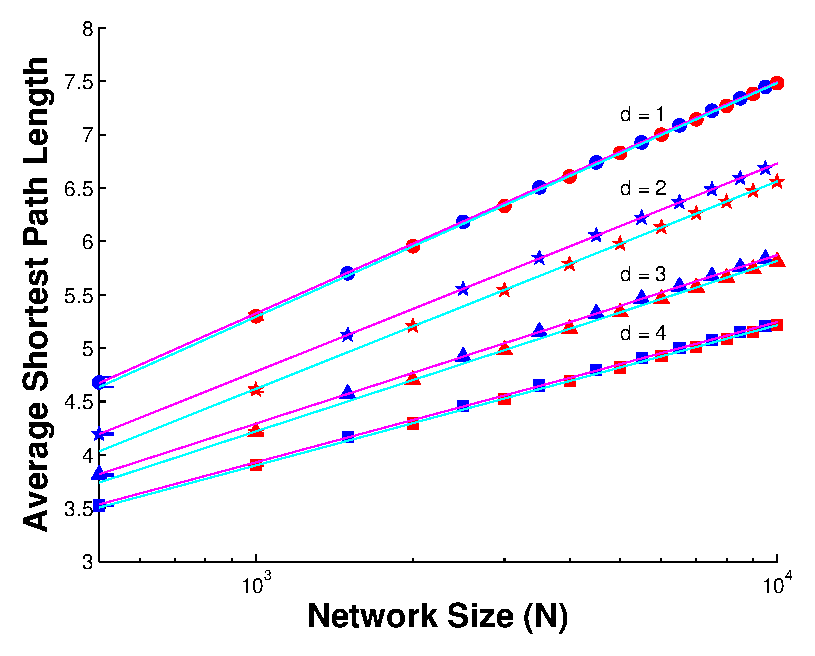
\includegraphics[width=\linewidth]{figures/figPLvsN.pdf}
\caption{\label{pathlength}Semilogarithmic plot of characteristic graph path length ($\ell$) shows the desired scaling, $\ell \sim \log N$. Note that in general the average shortest path is shorter in the higher dimensions. The blue points are for the Sphere Network Model while the red points are for the Plum Pudding Network Model ($alpha = d-1$ in both cases). Circles, starts, triangles and squares are respectively for $d = 1$,$2$,$3$, and $4$.}
\end{figure}

  \item \textbf{Clustering Coefficient:} The clustering coefficients in this model vary as we change the dimension of the embedding space, but in each case we find that for large $N$ the clustering approaches an asymptotic value. 
Results for $d = 1,2,3,4$ are displayed in Fig. \ref{clustN} with linear fits on the $N \geq 5000$ data to illustrate convergence to an $N$-invariant value.
Values for this $N$-invariant clustering are given as follows;
($d=1$): 0.44, ($d=2$): 0.29, ($d=3$): 0.16, ($d=4$): 0.09.
The higher dimensional cases also have this $N$-invariant clustering, and we find that as we increase dimension, clustering decreases (see Fig. \ref{clustdim} for more detail).

\begin{figure}
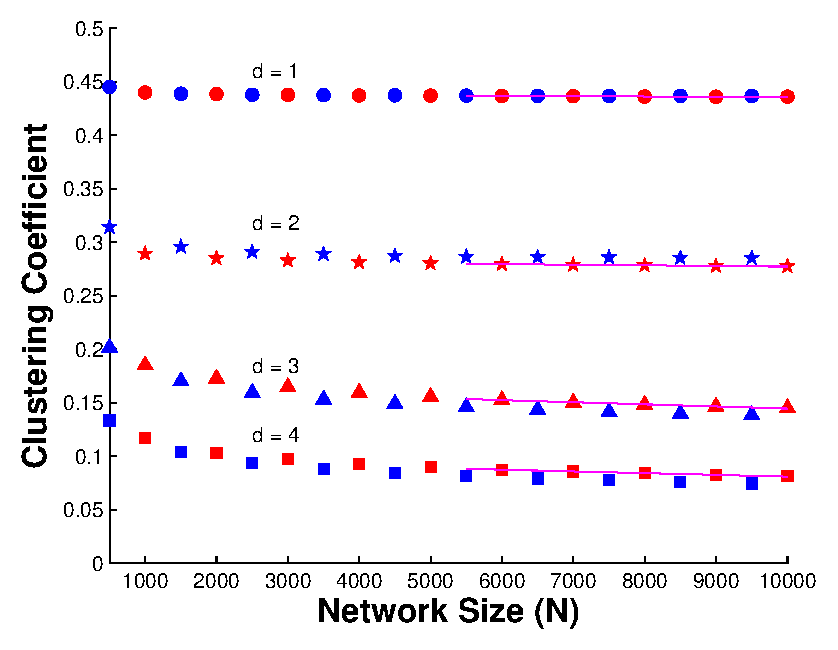
\includegraphics[width=\linewidth]{figures/figCvsN.pdf}
\caption{\label{clustN}Clustering coefficient vs. network size. The linear fits have approximately zero slope, showing that for large $N$ the clustering coefficient approaches a non-zero asymptote. The blue points are for the Sphere Network Model while the red points are for the Plum Pudding Network Model ($\alpha = d-1$ in both cases). Circles, starts, triangles and squares are respectively for $d = 1$,$2$,$3$, and $4$.}
\end{figure}

\end{itemize}
Thus we find that that the sphere model of a network growing on a $d$-sphere with geographic attachment preference leads to small-world networks.

\section{THE PLUM PUDDING NETWORK MODEL}
The Sphere Network Model described above has the feature that the geographical embedding region does not have an edge.
Thus we have also tested another model with different topology.
We call this second model the Plum Pudding Network Model.

We again model our nodes as a collection of negative point charges in $d$-dimensions.
The growth procedure is similar to the previous models; we place new nodes randomly in our volume and connect them to their $m$ nearest neighbors, where here we define nearest to be the Euclidean distance between the nodes.
Now, however, we regard the nodes as free to move in a unit radius, $d$-dimensional ball containing a uniform background positive charge density such that the total background charge in the sphere is equal and opposite to that of the $N$ network nodes.
Similar to our previous model, after adding a node with uniform probability density within the unit $d$-dimensional ball, we relax the charge configuration to a local energy minimum via the process,
\begin{equation}
d\textbf{x}_i/dt = \textbf{F}_i,\\
\textbf{F}_i = \sum_{j} (\textbf{x}_i - \textbf{x}_j)/|\textbf{x}_i-\textbf{x}_j|^{d-1} - N\textbf{x}_i,
\end{equation}
where $\textbf{x}_i$ is a $d$-dimensional vector, and the term $N\textbf{x}_i$ is due to the positive charge density.
The repulsive force between nodes ensures that they are spaced approximately equidistantly for large $N$ in a minimum potential configuration, while the cloud of positive charge ensures that the nodes remain in the sphere.

Due to the nature of Gauss's Law for any dimension $d$ the `force' of attraction between a node and the center of the background constant-density positive charge cloud is proportional to the value of the radial coordinate of the node.
This means that we can visualize this model as a collection of electrons all connected to the origin by springs (a harmonic potential) and interacting with each other via the dimensionally appropriate Couloumb force.  

We now consider the one-dimensional Plum Pudding Network Model on a line segment and compare it to the original Circle Model.
For the electrostatic problem on a one-dimensional line segment, we regard the node particles as charge sheets, which, through Gauss's law, leads to a constant separation-distance-independent repulsive force between electron pairs, thus the equilibrium for both the analogous $1$-d Sphere Network (i.e. Circle) and Plum Pudding Network Models yields equally spaced nodes. 
On the circle every node borders two internode intervals, while on the line segment, this is so for $(N-2)$ interior nodes with only the two boundary nodes bordering just one internode interval.
Thus as $N \to \infty$, the one-dimensional Plum Pudding Network Model is expected to yield results that are identical to those of the Circle Model.
Two fundamental properties of our one-dimensional models are that, when a new node is added, relaxation to equilibrium preserves the relative spatial ordering of nodes, and the equilibrium has uniform internodal spacing.
In contrast, for $d \geq 2$ the concept of linear ordering is absent.
In addition, for our $d \geq 2$ sphere and plum pudding topologies, exact, global regular-lattice positioning is not possible.
E.g., for $N \gg 1$ on a $2$-d sphere surface, it is known that, although equilibrium positioning through much of the area of the sphere is locally approximately a regular triangular lattice, the sphere's surface curvature leads to point and line defects in the triangular lattice pattern \cite{nelson}.
Thus a natural question is whether the $d = 1$ cases might have special properties that deviate from those for $d \geq 2$.

FIXME: Discuss Fig. \ref{clustdim} and hopefully explain $C \sim d^2$.

\begin{figure}
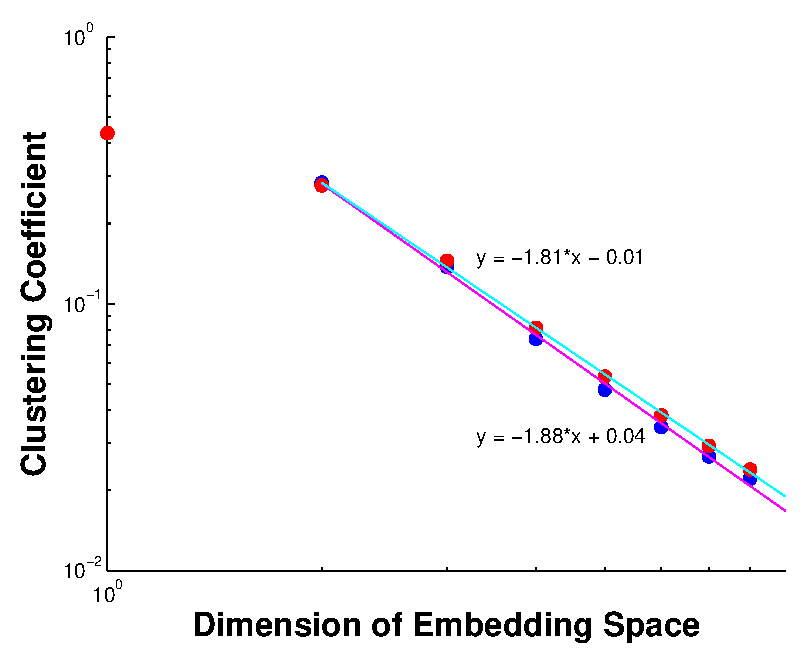
\includegraphics[width=\linewidth]{figures/figCvsD.pdf}
\caption{\label{clustdim}Log-log plot of asymptotic clustering coefficient versus dimension of embedding space reveals that for $d \geq 2$ the clustering ($C$) scales with $d^2$. This relationship, $C \sim d^2$ was found from the slopes of the linear fits. Blue points are for the Sphere Network Model while the red points are for the Plum Pudding Network Model ($\alpha = d-1$ in both cases).}
\end{figure}

\section{INVARIANT PROPERTIES}
Several important network features can be found analytically and for $N \gg 1$ do not depend on dimension and are the same for the Plum Pudding Network or Sphere Network Model.
A key observation in each of the following derivations is that, for large $N$, the probability that a newly added node will form an edge to any particular existing node is $m/N$ for all nodes.
This is because existing nodes are distributed approximately uniformly, and new nodes are placed randomly according to a uniform probability distribution.

\subsection{Degree Distribution}
\label{sub:degreedistribution}
Here we show that for each considered model, we produce the same master equation governing the evolution of the degree distribution (in particular the master equation for the degree distribution in \cite{ozik2004}).  
This master equation is not specific to the spatial structure of the network and appears, in various forms, in other network models, such as the Deterministic Uniform Random Tree of Ref. \cite{zhang2008topologies}.

We define $\hat{G}(k,N)$ to be the number of nodes with degree $k$ when we are at time $N$ (i.e. when the system has $N$ nodes).
When a node is added to the network it is initially connected to its $m$ nearest neighbors, so initially (upon creation) $k = m$ for each node, meaning that $\hat{G}(k,N) = 0 \text{ for } k < m$.
Since each existing node is equally likely to be chosen to be connected to the new node, there is a $m/N$ probability that any given node with have its degree incremented by 1.
Averaging $\hat{G}(k,N)$ over all possible random node placements we get a master equation for the time evolution of $G(k,N)$, the average of $\hat{G}(k,N)$ over all possible randomly grown networks;
\begin{equation}
G(k,N+1) = G(k,N) - \frac{m}{N}G(k,N) + \frac{m}{N}G(k-1,N) + \delta_{km},
\end{equation}
\noindent where $\delta_{km}$ is the Kronecker delta function.
The first term on the right is the expected number of nodes with degree $k$ at time $N$.
The second term is the expected number of nodes with degree $k$ at time $N$ that get promoted to degree $k+1$.
The third term is the expected number of nodes with degree $k-1$ at time $N$ that get promoted to degree $k$.
The last term on the right is the new node with degree $m$.

It was shown by Ozik et al. \cite{ozik2004} that this master equation leads to an exponentially decaying degree distribution with an asymptotically $N$ invariant form $H(k) = \lim_{N \to +\infty} G(k,N)/N$ given by
\begin{equation}\label{degeq}
H(k) = \frac{1}{m+1}\left(\frac{m}{m+1}\right)^{k-m}.
\end{equation}
\noindent for $k \geq m$ and $H(k) = 0$ for $k < m$.

\begin{figure}
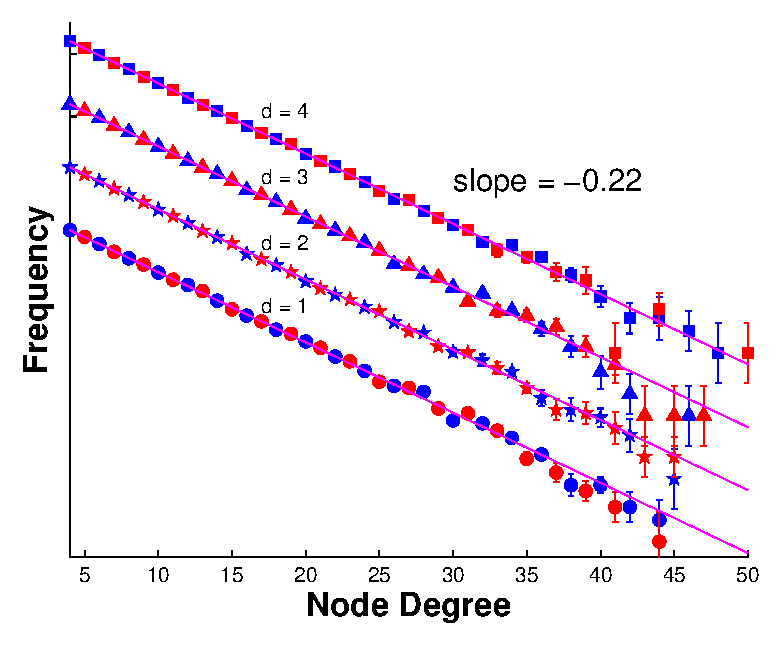
\includegraphics[width=\linewidth]{figures/figDegDist.pdf}
\caption{\label{degdist}Semilogarithmic graph of the degree distribution for 8 models with $N = 10000$ and $m = 4$ compared to the theory in Eq. \eqref{degeq}. The slope of -0.22 agrees with the theoretical slope of $\log \frac{m}{m+1} = \log \frac{4}{5} \approx -0.22$. The blue points are for the Sphere Network Model while the red points are for the Plum Pudding Network Model. Circles, stars, triangles, and squares are respectively for $d=1$, $2$, $3$, and $4$. Note that an arbitrary linear offset was used to separate data for visualization and thus values on the y-axis are only relative.}
\end{figure}

Interestingly, this exponentially decaying degree distribution comes only from the growth process and the uniform probability of attaching new links to existing nodes.  
As seen in Fig. \ref{degdist}, for $m = 4$, $N = 10^4$, with $d = 1,2,3,4$, Eq. \eqref{degeq} is well-satisfied by numerical simulations of both the Sphere Network (blue points) and Plum Pudding Network (red points) Models.

\subsection{Mean Degree as a Function of Node Age}
We seek an expression for the expected degree $k(y,N)$ of a node that has existed for $y$ time steps given that the network size is $N$ ($y < N$).
Each node connects to its $m$ nearest neighbors upon creation, and the probability of incrementing the degree of the node is $m/N$, when the size of the network is $N$.
Thus we obtain 
\begin{equation}\label{ageeq}
\begin{split}
k(y,N)& = m + m\sum_{n=N-y+1}^{N} \frac{1}{n}\\
      & \approx m + m \log \frac{N}{N-y} + \mathcal O\left(\frac{1}{N^2}\right)
\end{split}
\end{equation}
 
Once again, since this derivation uses only the assumption that each node has an equal chance each time step to have its degree incremented, the result holds for both of the models discussed here.
This represents a specific example of the fact that in dynamically growing networks, older nodes are preferentially connected to one another as discussed in \cite{reallyrandom}.
\begin{figure}
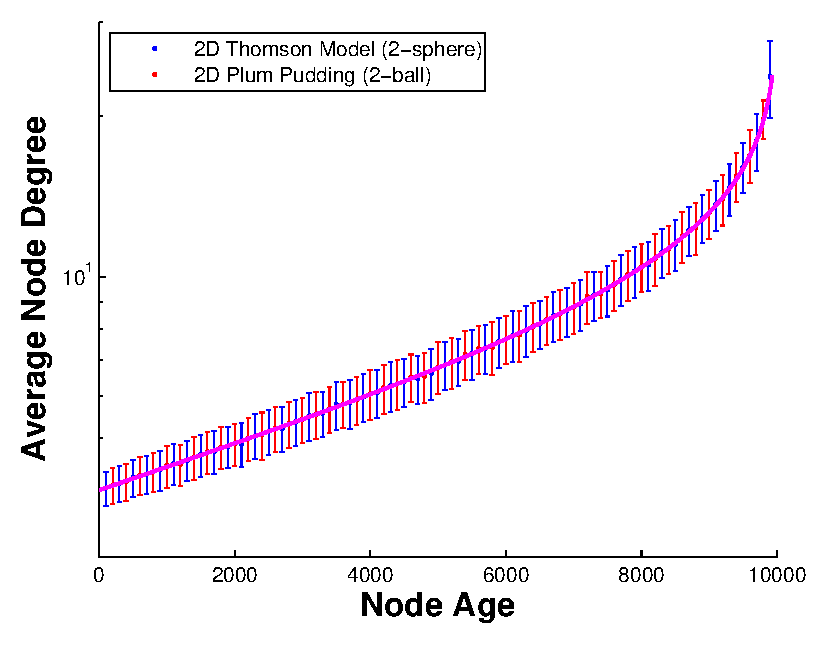
\includegraphics[width=\linewidth]{figures/figDvsAge.pdf}
\caption{\label{degage}Semilogarithmic graph of the mean degree vs the node age for two of the explored models with $N = 10000$ and $m = 4$. The magenta line is the theory in Eq. \eqref{ageeq} and the error bars are the standard deviation of the average over 10 simulated networks}
\end{figure}
Numerical simulations of the mean degree as a function of node age, Fig. \ref{degage}, demonstrate that Eq. \eqref{ageeq} is satisfied for both the Sphere Network (blue points) and Plum Pudding Network (red points) Models.
Results are only presented for the $2$-dimensional case for simplicity, but the Eq. \eqref{ageeq} has no dependence on the embedding space, and thus holds for other dimensions as well.

\subsection{Dependence on $\alpha$, the force exponent}
\label{sub:forcelaw}
In calculating the gradients for the gradient-descent algorithm, we use a force law motivated by electrostatics, with the force on node $i$ given by 
\begin{equation}
F_i \sim \sum_{i \neq j} \frac{1}{|\textbf{x}_i - \textbf{x}_j|^{\alpha}}, 
\end{equation}
with $\alpha = d-1$ in a $d$-dimensional space and $\textbf{x}_i$ the position vector of node $i$.
Using a force familiar from electrostatics serves a dual purpose, (i) it turns an otherwise difficult problem into a familiar one for which literature is plentiful, and (ii) it provides physical motivation for the movement and dynamics of the nodes in our networks.
Furthermore, the choice of $\alpha = d-1$ was found to minimize computational time while still achieving the equalization desired compared to larger values of $\alpha$.
Nevertheless, we find different values of $\alpha$ do not produce significant changes to the structure of our network models.
Larger values of $\alpha$ simply add computational difficulty to the problem, but if the gradient descent method is implemented with the correct parameters, distinct values of $\alpha$ lead to the same network properties as the models described previously.
In Fig. \ref{forcelaw} we demonstrate agreement in the clustering coefficient for various values of $\alpha$ for the $d=2$ case in the Sphere Network Model.
Thus we find that our results apply not only to nodes behaving as negative charges, but to any system where nodes interact through a distatnce-dependent monotonic repulsive force.

%\begin{figure}
%\includegraphics[width=\linewidth]{figures/CvsFLaw.pdf}
%\caption{\label{forcelaw}Clustering coefficient vs force exponent $\alpha$ for the $d = 2$ Sphere Network Model, indicating that the network properties generated by this model are independent of the choice of $\alpha$.}
%\end{figure}

\section{CONCLUSION}
We expanded upon the work presented in \cite{ozik2004} to generate small-world networks embedded in more general spaces.
By allowing nodes to move in space, our models provide a realistic model of how small-world networks can emerge from a growing collection of dynamically interacting and locally constrained vertices.  
Furthermore, we find that the dimension of the space in which the nodes are embedded determines how they cluster, in particular we find that the clustering coefficient C scales as $C \sim 1/d^{-2}$ for a $d$-dimensional space.
We hope these finding will spark interest in dynamic spatial networks, as most real world networks grow and shift position in some underlying space.

\nocite{*}
\bibliography{grownet}

\end{document}

